\chapter{Metodolog'ia de desarrollo y calid'ad}
\section{An'alisis}
\begin{center}

\end{center}

Metodología propuesta: Xtreme programming
Justificación: la metodología usada es Xtreme programming ya que es el más destacado de los procesos ágiles de desarrollo de software, esta metodología nos ofrece una gran cantidad de ventajas como:
\begin{itemize}
\item Tener una programación totalmente organizada.
\item Fomenta la comunicación entre los clientes y los desarrolladores, este punto es muy importante ya que si no hay una buena comunicación entre los desarrolladores y el cliente va a ser muy difícil que el proyecto cumpla con los requisitos establecidos por el cliente.
\item Se hacen pruebas continuas durante el proyecto. Así se obtendrá una menor taza de errores en el proyecto.
\item Es muy recomendable en utilizarlo en proyectos cortos.
\item Permite ahorrar mucho tiempo y dinero.
\end{itemize}

La metodología Xtreme programming tiene muchas ventajas establece las mejores prácticas de Ingeniería de Software en los desarrollos de proyectos, mejora la productividad de los proyectos y garantiza la calidad del software, haciendo que supere las expectativas del cliente.

\subsection{Requerimientos funcionales}
\begin{itemize}
\item El sistema contara  con un login de Usuario
\item El sistema permite el registro de usuarios nuevos
\subitem Permite registrar usuarios mediante Gmail
\item El menu principal tendra acceso a los Temas y a los juegos de la aplicaión
\item La informcación se dividira en Temas de estudio 
\item Cada tema contara con una evaluación.
\item El menu de juegos tendra 3 formas de juego.
\subitem Cuestionario.
\subitem Encuentra el Error.
\subitem Completa la sintaxis.
\item Dentro del menu de juego podras entrar al modulo de puntuaciones.
\item El menu de Temas mostrara la puntuacion mas alta que tengas de cada Tema.
\end{itemize}

\subsection{Requerimientos no funcionales}
\begin{itemize}
\item Toda la funcionalidad del sistema debe responder al usuario en menos de 5 segundos.
\item El sistema debe mostrar mensajes de error que sean informativos y orientados a usuario final.
\subitem El sistema debe poseer interfaces gráficas bien formadas
\item La aplicación no podra ocupar más de 2 GB de espacio en disco.
\end{itemize}
\section{Dise'no}
\subsection{Casos de uso}
\begin{center}
\begin{figure}[H]
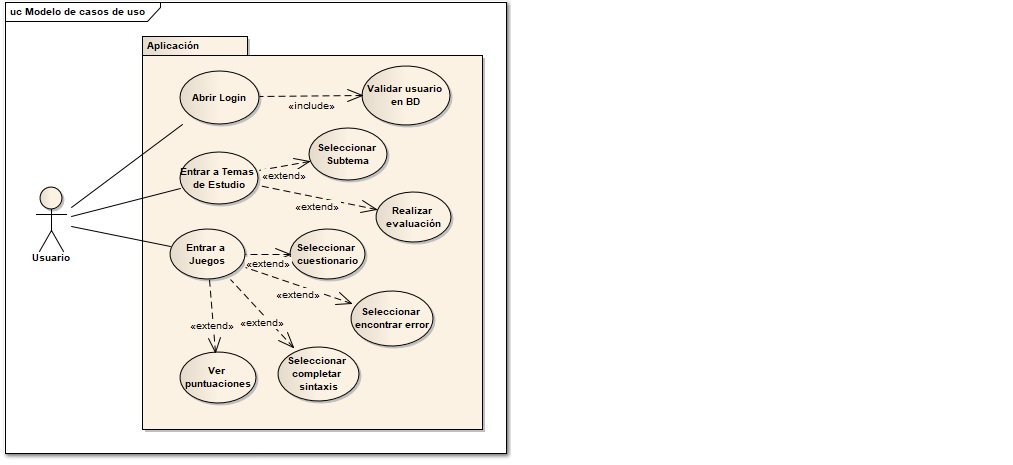
\includegraphics[scale=0.8]{img/uso.jpg} 
\caption{Diagrama de Casos de uso.}
\end{figure}
\end{center}
\subsection{Mockup}
\begin{center}
\begin{figure}[H]
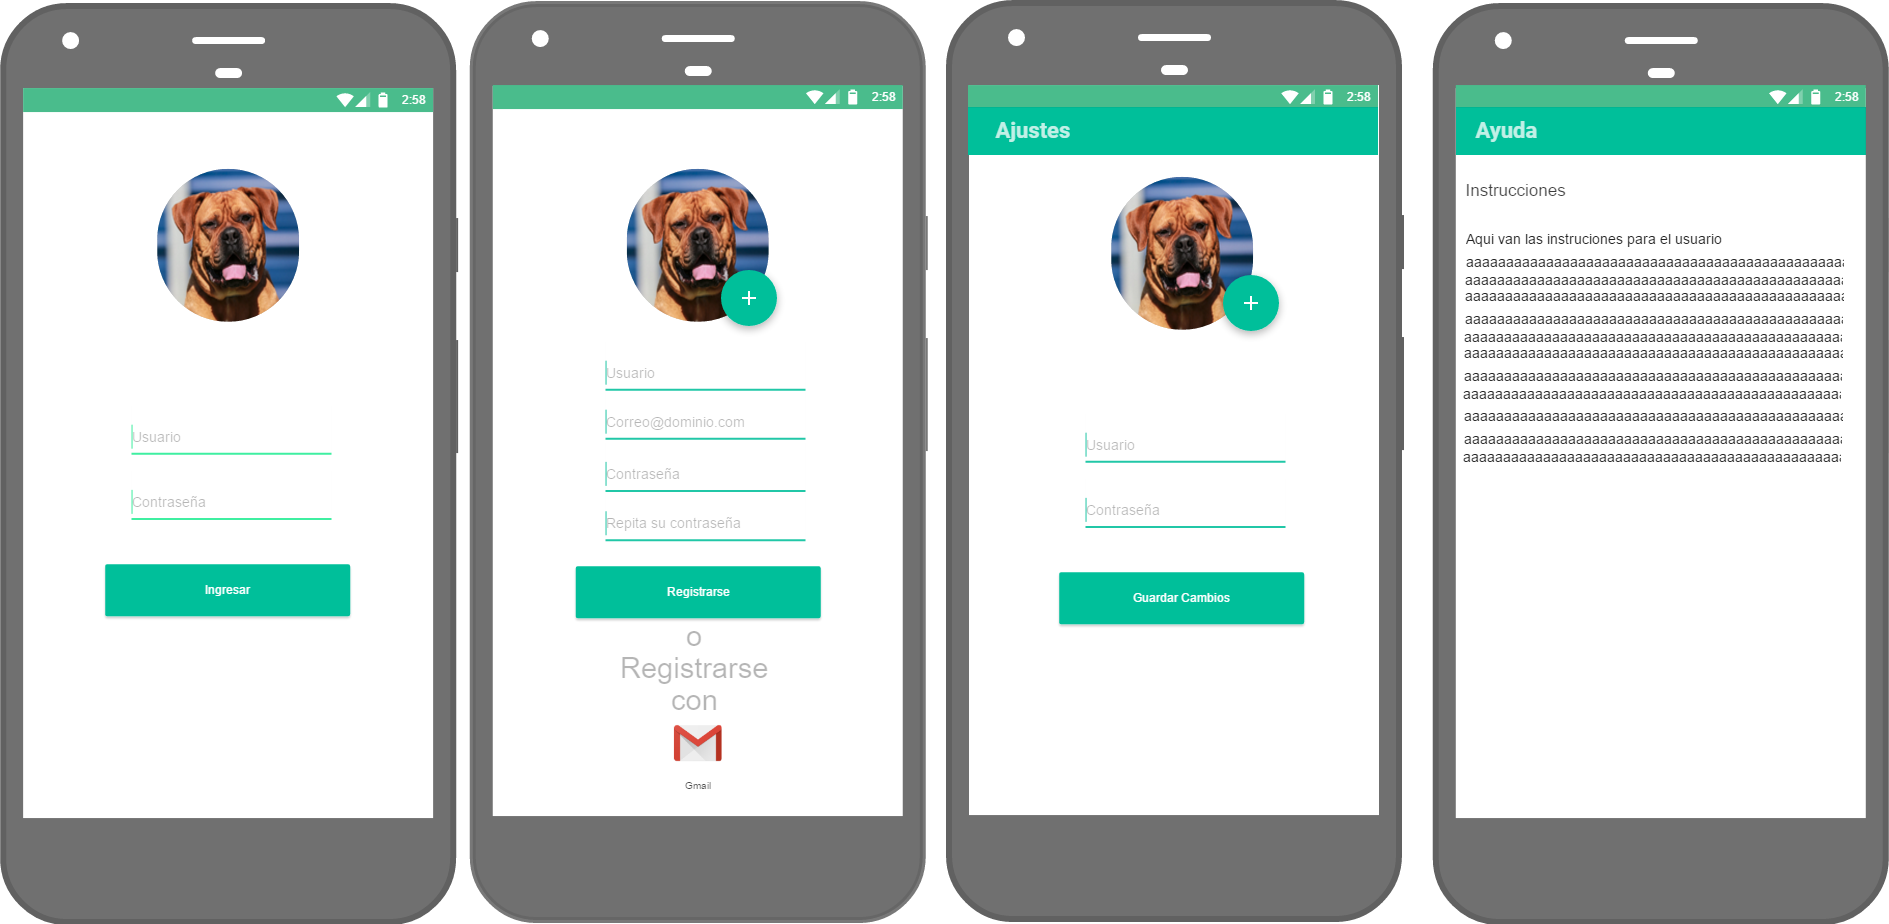
\includegraphics[scale=0.2]{img/m1.png} 
\caption{Pantallas de inicio de sesión y sección de ayuda}
\end{figure}
\end{center}

\begin{center}
\begin{figure}[H]
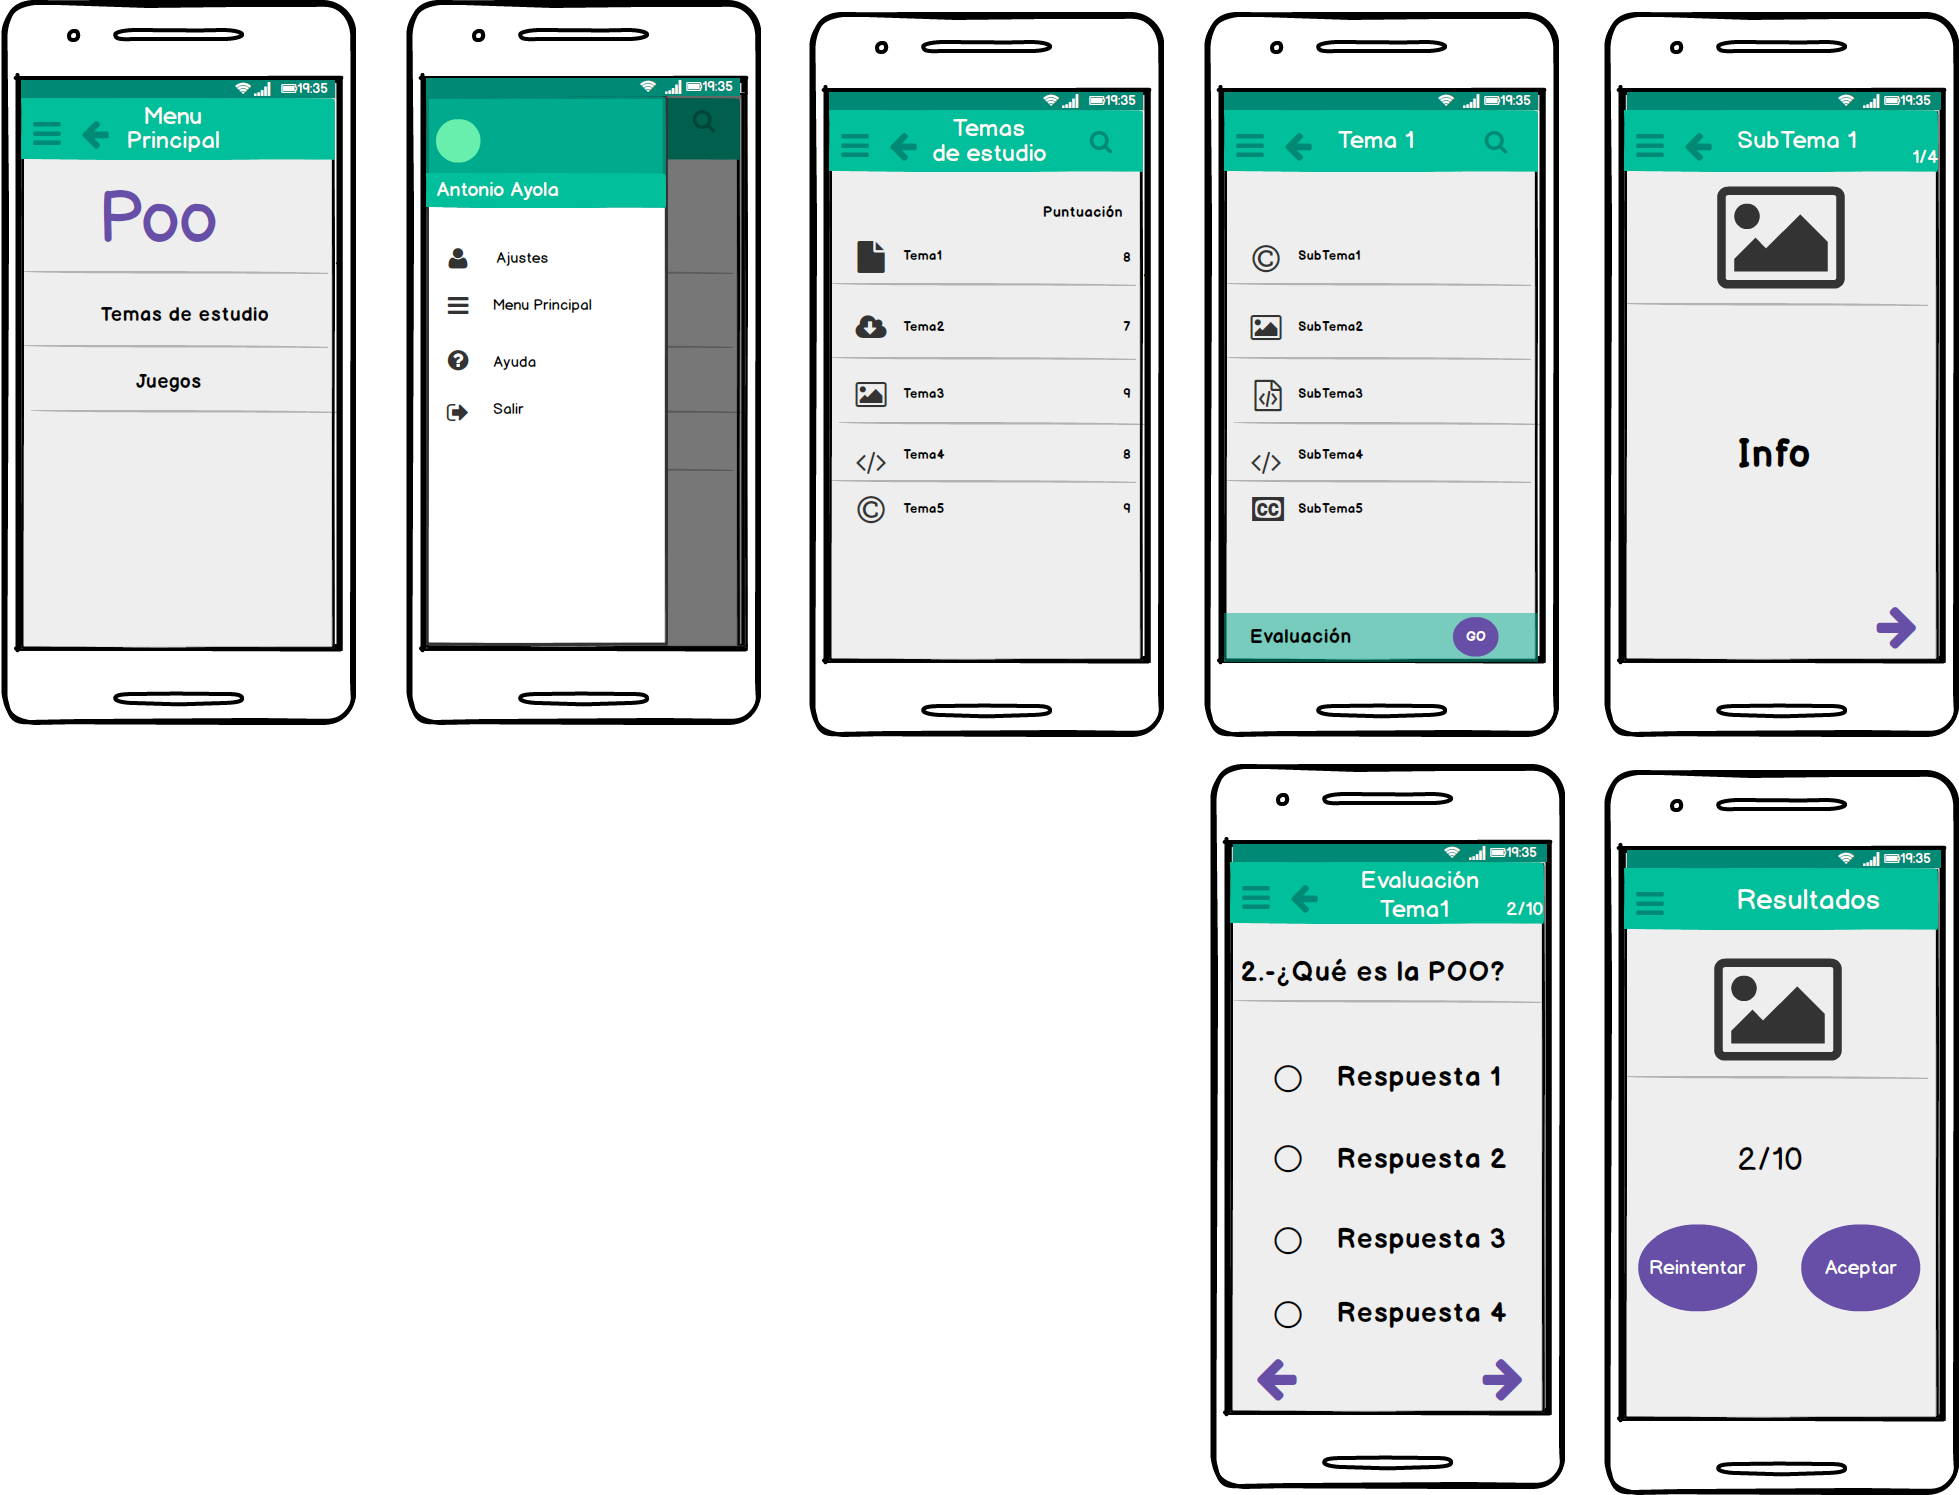
\includegraphics[scale=0.3]{img/m2.png} 
\caption{Pantallas del menú principal, temas, subtemas y evaluación.}
\end{figure}
\end{center}

 
\begin{figure}[H]
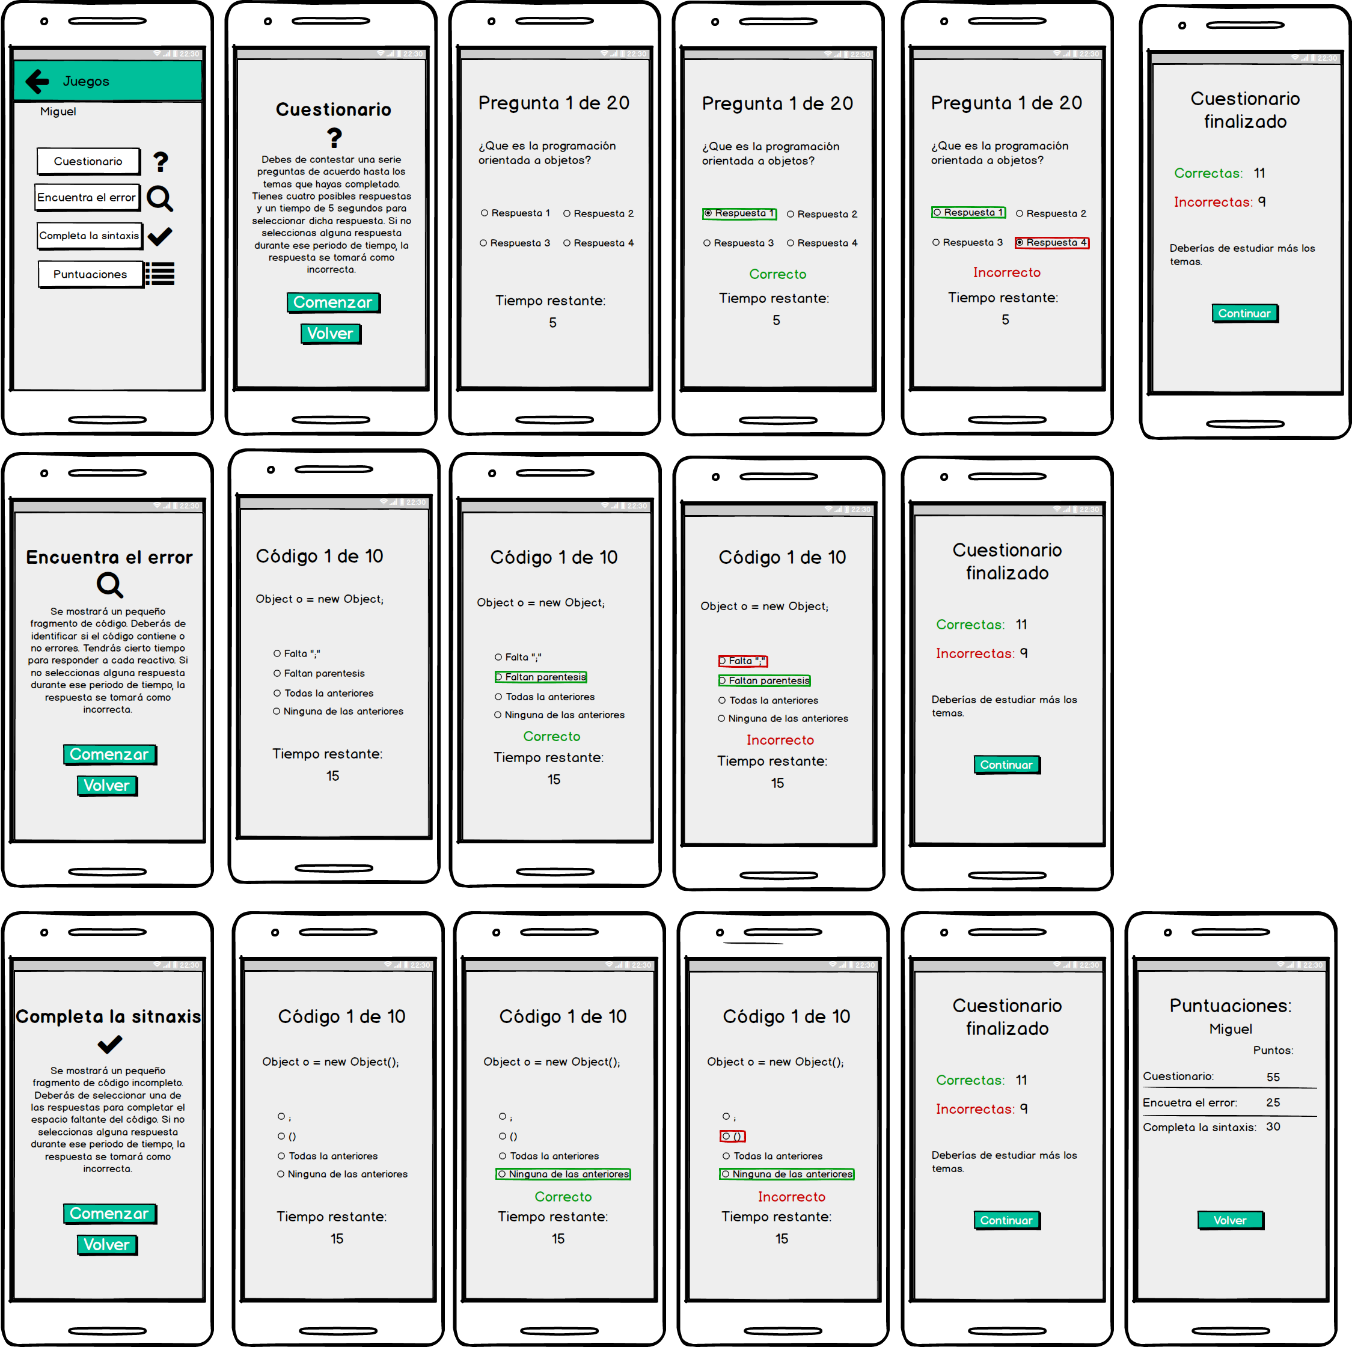
\includegraphics[scale=0.9]{img/m3.png} 
\caption{Pantallas de la sección de juegos}
\end{figure}


\subsection{Diagrama de navegabilidad}
\begin{figure}[H]
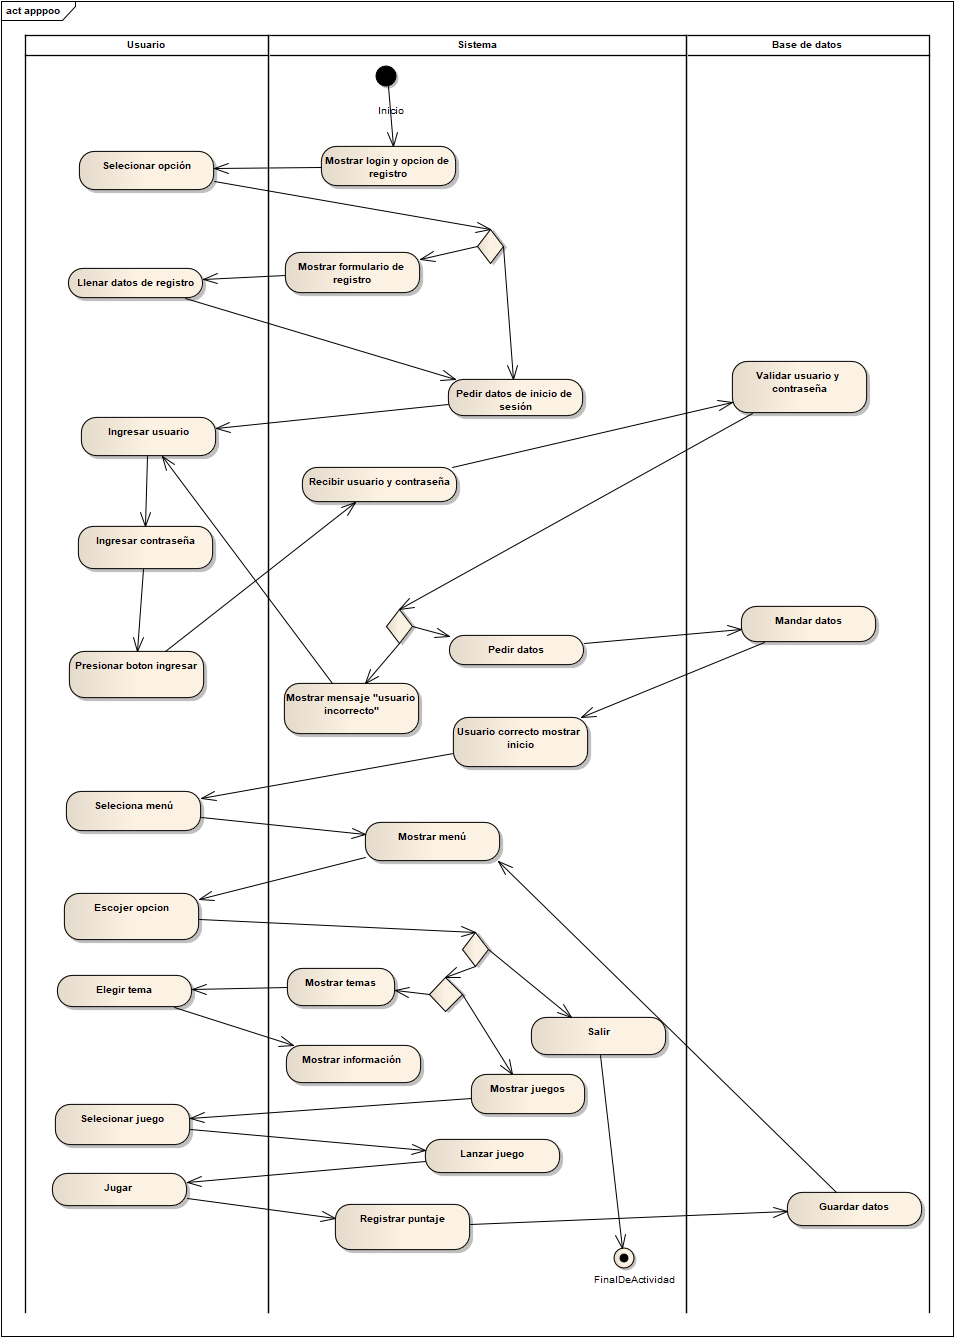
\includegraphics[scale=0.2]{img/diagrama.png} 
\caption{Diagrama de navegabilidad}
\end{figure}

\subsection{Diagrama entidad-relaci'on}

\section{Programaci'on}

\section{Implementaci'on}

\section{Cronograma}
\begin{center}
\begin{figure}[H]
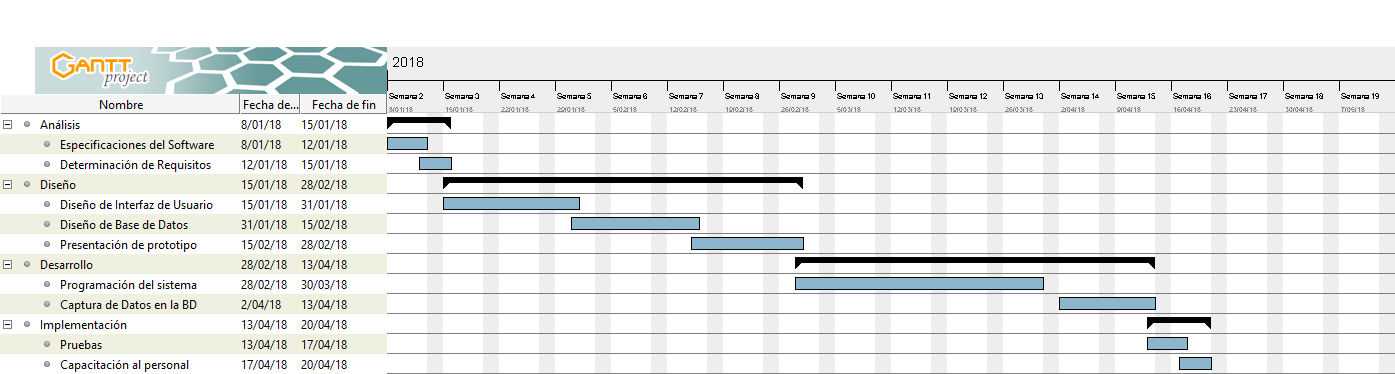
\includegraphics[scale=0.3]{img/gant.jpg} 
\caption{Diagrama de Gantt}
\end{figure}
\end{center}

\section{Pruebas}
	\begin{table}[H]
\centering
\caption{Pruebas}
\label{my-label}
\begin{tabular}{lllll}
Caso de Prueba\# & Caso de Prueba                                         & Pasos                                                                                                          & Resultado &  \\
1                & Login permite acceso a usuario correcto                & \begin{tabular}[c]{@{}l@{}}-Ingresar Usuario correcto\\ -Ingresar contraseña correcta\\ -Ingresar\end{tabular} &           &  \\
2                & Login no permite acceso a usuario incorrecto           & \begin{tabular}[c]{@{}l@{}}-Ingresar Usuario correcto\\ -Ingresar contraseña correcta\\ -Ingresar\end{tabular} &           &  \\
3                & El menu de temas muestra correctamente todos los temas & \begin{tabular}[c]{@{}l@{}}-Menu Principal\\ -Seleccionar Temas de estudio\end{tabular}                        &           & 
\end{tabular}
\end{table}

